\documentclass[12pt, a4paper]{article}

% Codificação e Língua
\usepackage[utf8]{inputenc}
\usepackage[T1]{fontenc}

% Layout
\usepackage[top=3cm, bottom=2cm, left=3cm, right=2cm]{geometry}
\usepackage{setspace}
\onehalfspacing

% Cores
\usepackage[dvipsnames, table]{xcolor}
\definecolor{ufrn-blue}{RGB}{0, 58, 113}
\definecolor{code-bg}{RGB}{245, 247, 250}
\definecolor{frame-gray}{RGB}{180, 180, 180}
\definecolor{accent}{RGB}{0, 100, 180}

% Gráficos e diagramas
\usepackage{tikz}
\usetikzlibrary{arrows.meta, positioning, shapes.geometric, fit, backgrounds, calc, shadows}

% Listagens de código
\usepackage{listings}
\lstdefinestyle{telchain}{
  backgroundcolor=\color{code-bg},
  basicstyle=\ttfamily\small,
  keywordstyle=\color{ufrn-blue}\bfseries,
  commentstyle=\color{gray}\itshape,
  stringstyle=\color{Maroon},
  breaklines=true,
  frame=single,
  rulecolor=\color{frame-gray},
  numbers=left,
  numberstyle=\tiny\color{gray},
  tabsize=4,
  showstringspaces=false,
  captionpos=b
}
\lstset{style=telchain}

% Tabelas
\usepackage{booktabs}
\usepackage{tabularx}
\usepackage{longtable}
\usepackage{multirow}
\usepackage{array}

% Cabeçalho/Rodapé
\usepackage{fancyhdr}
\pagestyle{fancy}
\fancyhf{}
\fancyhead[L]{\small\textcolor{ufrn-blue}{\textbf{TelChain}} --- Especificação da Aplicação}
\fancyhead[R]{\small DIM0438 --- Redes de Computadores}
\fancyfoot[C]{\small\thepage}
\renewcommand{\headrulewidth}{0.4pt}

% Hyperlinks
\usepackage[hidelinks, colorlinks=true, linkcolor=ufrn-blue, urlcolor=accent]{hyperref}

% Outros pacotes 
\usepackage{graphicx}
\usepackage{enumitem}
\usepackage{float}
\usepackage{caption}
\usepackage{subcaption}
\usepackage{amsmath}
\usepackage{amssymb}
\usepackage{tcolorbox}
\tcbuselibrary{skins, breakable}
\usepackage{dirtree}

% Caixa de destaque
\newtcolorbox{infobox}[1][]{
  enhanced, breakable,
  colback=blue!5!white, colframe=ufrn-blue,
  fonttitle=\bfseries, title=#1,
  left=6pt, right=6pt
}

\newtcolorbox{warnbox}[1][]{
  enhanced,
  colback=orange!8!white, colframe=orange!70!black,
  fonttitle=\bfseries, title=#1,
  left=6pt, right=6pt
}

% -----------------------------------------------------------------
%  Documento
% -----------------------------------------------------------------
\begin{document}

% Capa
\begin{titlepage}
\centering
\vspace*{0.5cm}

{\large\textbf{Universidade Federal do Rio Grande do Norte}}\\[0.2cm]
{\large Departamento de Informática e Matemática Aplicada}\\[0.2cm]
{\large Bacharelado em Tecnologia da Informação (BTI)}\\[0.8cm]

\noindent\rule{\linewidth}{1.5pt}
\vspace{0.4cm}

{\Huge\bfseries\textcolor{ufrn-blue}{TelChain}}\\[0.3cm]
{\Large Telemetria de Sensores IoT com Registro em Blockchain}\\[0.3cm]
{\large\textit{Especificação da Aplicação Cliente/Servidor}}

\vspace{0.4cm}
\noindent\rule{\linewidth}{1.5pt}

\vspace{1.5cm}

\begin{tabular}{ll}
\textbf{Disciplina:}  & DIM0438 --- Redes de Computadores \\[4pt]
\textbf{Professor:}   & Augusto José Venâncio Neto \\[4pt]
\textbf{Aluna:}       & Yasmin Giordano Santos \\[4pt]
\textbf{Matrícula:}   & 20240012578 \\
\end{tabular}

\vfill

{\small Natal -- RN, \the\year}
\end{titlepage}

% Sumário
\tableofcontents
\newpage

\section{Visão Geral do Projeto}

A \textbf{TelChain} é uma aplicação cliente/servidor que combina telemetria ambiental com uma blockchain didática.
Sensores IoT simulados enviam periodicamente leituras de temperatura, umidade e pressão atmosférica por meio de um
protocolo proprietário baseado em sockets TCP. Enquanto isso, o servidor central, após autenticar cada dispositivo, agrupa as
leituras em transações e as registra em blocos encadeados protegidos por Prova de Trabalho (PoW), assegurando a
imutabilidade dos dados. Por fim, clientes do tipo \emph{Dashboard} operam em modo interativo, podendo inspecionar a cadeia
sob demanda e receber notificações \emph{push} de novos blocos e transações em tempo real, além de terem a capacidade de auditar a
integridade de toda a estrutura.

\subsection{Motivação}
A ideia para o projeto surgiu do interesse em explorar a integração entre blockchain e a Internet das Coisas,
bem como do aprofundamento nos fundamentos de comunicação por sockets em Java. Mais especificamente, a escolha de um cenário de
telemetria ambiental permite exercitar, em um único sistema, os conceitos de protocolo de rede proprietário,
concorrência com múltiplos clientes e registro imutável de dados por meio de uma cadeia de blocos
simplificada com prova de trabalho.

\subsection{Repositório}

O código-fonte do projeto está organizado conforme ilustra a Figura~\ref{fig:dirtree}. 
Na raiz situa-se o \texttt{build.sh}, encarregado da compilação e empacotamento, 
enquanto o código Java fica em \texttt{src/telchain/}, dividido em três pacotes: 
\texttt{blockchain} com a lógica de integridade dos dados, 
\texttt{client} com as interfaces de sensor e \emph{dashboard}, e 
\texttt{server} com a implementação do ponto central de comunicação.


\begin{figure}[H]
\centering
\begin{tcolorbox}[colback=code-bg, colframe=black, boxrule=0.4pt, width=0.7\textwidth, arc=0mm]
\dirtree{%
.1 telchain/.
.2 build.sh.
.2 src/.
.3 telchain/.
.4 blockchain/.
.5 Block.java.
.5 Blockchain.java.
.5 Transaction.java.
.4 client/.
.5 DashboardClient.java.
.5 SensorClient.java.
.4 server/.
.5 ClientHandler.java.
.5 TelChainServer.java.
}
\end{tcolorbox}
\caption{Estrutura de diretórios do projeto TelChain.}
\label{fig:dirtree}
\end{figure}

\section{Arquitetura da Aplicação}

\subsection{Visão Arquitetural}

A aplicação adota uma arquitetura estrela centralizada (\emph{hub‑and‑spoke}): todos
os clientes se conectam exclusivamente ao servidor, que atua como o \emph{hub}
central, enquanto sensores e \emph{Dashboards} funcionam como \emph{spokes}. Em 
outras palavras, não há comunicação direta entre clientes, toda mensagem sempre 
passa pelo \emph{hub}. Esse aspecto, além de seguir a especificação dada para o 
projeto, simplifica o protocolo e elimina a necessidade de um mecanismo de consenso 
distribuído.

\begin{figure}[H]
\centering
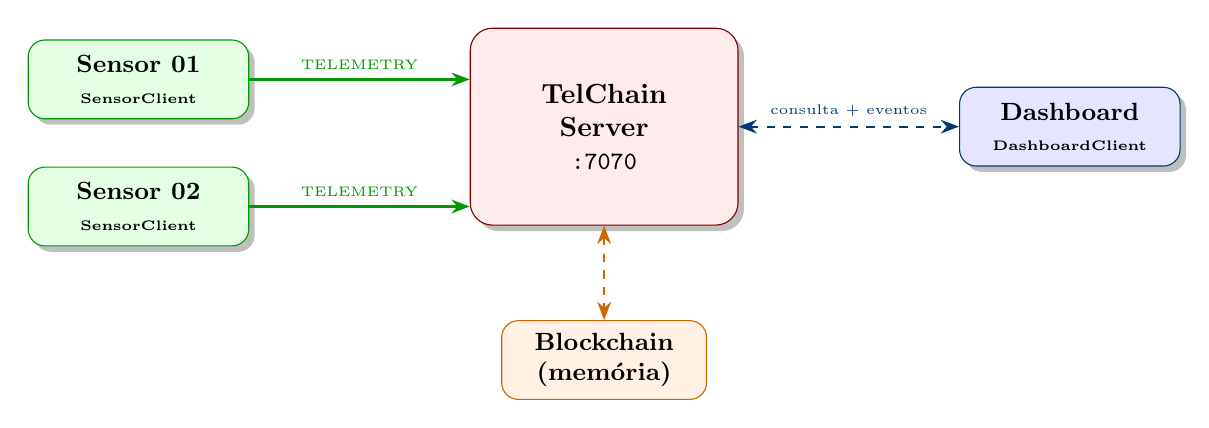
\begin{tikzpicture}[
  node distance=1.8cm and 2.8cm,
  sensor/.style={draw=green!60!black, fill=green!10, rounded corners=6pt,
                 minimum width=2.8cm, minimum height=1cm, align=center,
                 font=\small\bfseries, drop shadow},
  dashnode/.style={draw=ufrn-blue, fill=blue!10, rounded corners=6pt,
               minimum width=2.8cm, minimum height=1cm, align=center,
               font=\small\bfseries, drop shadow},
  server/.style={draw=Maroon, fill=red!8, rounded corners=8pt,
                 minimum width=3.4cm, minimum height=2.5cm, align=center,
                 font=\bfseries, drop shadow},
  blockchain/.style={draw=orange!80!black, fill=orange!10, rounded corners=6pt,
                     minimum width=2.6cm, minimum height=1cm, align=center,
                     font=\small\bfseries},
  arr/.style={-Stealth, thick},
  darr/.style={Stealth-Stealth, thick, dashed},
]

% Servidor (centro)
\node[server, anchor=center] (srv) {TelChain\\Server\\{\small\ttfamily :7070}};

% Sensores (esquerda)
\node[sensor, left=2.8cm of srv, yshift=0.6cm] (s1) {Sensor 01\\{\tiny SensorClient}};
\node[sensor, below=0.6cm of s1] (s2) {Sensor 02\\{\tiny SensorClient}};

% Dashboard (direita)
\node[dashnode, right=2.8cm of srv] (d1) {Dashboard\\{\tiny DashboardClient}};

% Blockchain (abaixo do servidor)
\node[blockchain, below=1.2cm of srv] (bc) {Blockchain\\(memória)};

% Setas sensores → servidor
\draw[arr, green!60!black] (s1.east) -- (srv.west |- s1.east) node[midway, above, font=\tiny]{TELEMETRY};
\draw[arr, green!60!black] (s2.east) -- (srv.west |- s2.east) node[midway, above, font=\tiny]{TELEMETRY};

% Setas servidor → dashboards (eventos push)
\draw[darr, ufrn-blue] (srv.east |- d1.west) -- node[above, font=\tiny]{consulta + eventos} (d1.west);

% Servidor ↔ Blockchain
\draw[darr, orange!80!black] (srv.south) -- (bc.north);

\end{tikzpicture}
\caption{Arquitetura geral do TelChain -- sensores publicam, servidor persiste na blockchain
         e \emph{dashboards} monitoram via push/pull.}
\label{fig:arch}
\end{figure}

\subsection{Componentes Principais}

A composição do sistema pode ser resumida como um conjunto de partes que 
cooperam entre si para realizar a coleta, o registro imutável e o monitoramento dos 
dados. A organização desses componentes espelha a arquitetura cliente/servidor e a 
separação entre a lógica de rede, o núcleo da blockchain e as interfaces de usuário, 
conforme detalhado na Tabela~\ref{tab:components}.

\begin{table}[H]
\centering
\caption{Componentes do sistema TelChain.}
\label{tab:components}
\begin{tabularx}{\linewidth}{lX}
\toprule
\textbf{Componente} & \textbf{Responsabilidade} \\
\midrule
\texttt{TelChainServer}  & Aceita conexões TCP na porta 7070; autentica clientes; delega o tratamento de cada conexão a um \texttt{ClientHandler}; agenda a selagem periódica de blocos a cada 30 s. \\
\addlinespace
\texttt{ClientHandler}   & Executa em thread própria; parseia o protocolo TelChain; despacha comandos; controla inscrições de eventos por cliente. \\
\addlinespace
\texttt{Blockchain}      & Estrutura de dados encadeada e thread-safe; gerencia o pool de transações pendentes; sela blocos automaticamente ao atingir 5 transações ou por gatilho do timer. \\
\addlinespace
\texttt{Block}           & Representa um bloco imutável; calcula a raiz de Merkle das transações; realiza a Prova de Trabalho (prefixo \texttt{"00"} no hash SHA-256). \\
\addlinespace
\texttt{Transaction}     & Value object imutável; armazena leitura de telemetria; calcula o hash SHA-256 de seus campos. \\
\addlinespace
\texttt{SensorClient}    & Simula sensor IoT com random walk gaussiano; envia \texttt{TELEMETRY} periodicamente; faz ping a cada 10 envios. \\
\addlinespace
\texttt{DashboardClient} & Interface interativa para auditoria; mantém thread leitora para receber eventos push; oferece comandos \texttt{chain}, \texttt{verify}, \texttt{block N}, \texttt{stats}, etc. \\
\bottomrule
\end{tabularx}
\end{table}

\subsection{Concorrência}

Para se proteger, o servidor adota o modelo \emph{thread-per-client}, criando uma nova \texttt{Thread} e 
um \texttt{ClientHandler} dedicado para cada conexão aceita, o que mantém o loop de 
aceitação desimpedido. Já a consistência da \texttt{Blockchain} é garantida por métodos 
\texttt{synchronized} em todas as operações mutantes, além da adoção de 
\texttt{CopyOnWriteArrayList} pela lista de clientes ativos para que iterações de 
\emph{broadcast} não sofram com modificações concorrentes. Por fim, a selagem periódica de blocos é confiada a um 
\texttt{ScheduledExecutorService} de thread única, que dispara o fechamento da \emph{pool} a 
cada 30 segundos sem interferir no tratamento de requisições.


\section{Estrutura da Blockchain}

\subsection{Transação (\textit{Transaction})}

A transação é a unidade atômica de dados que trafega do sensor até a blockchain.
Ela representa uma leitura ambiental pontual e imutável, cuja integridade é
garantida por um hash criptográfico calculado no momento da criação. Uma vez
incluída em um bloco, a transação torna-se parte permanente do registro
distribuído, podendo ser auditada a qualquer momento por um \emph{Dashboard}.

Cada leitura de telemetria gera uma transação com os campos:
\[
  \mathrm{TX} = \langle \mathit{deviceId},\ \mathit{temperature},\ \mathit{humidity},\ \mathit{pressure},\ \mathit{timestamp},\ \mathit{hash} \rangle
\]

Já o hash é calculado como:
\[
  \mathit{hash} = \mathrm{SHA\text{-}256}\!\left(\mathit{deviceId}\,\|\,\mathit{temp}\,\|\,\mathit{hum}\,\|\,\mathit{pres}\,\|\,\mathit{ts}\right)
\]

\subsection{Bloco (\textit{Block})}

O bloco é a unidade de agrupamento que sela as transações pendentes e as incorpora
definitivamente à cadeia. Cada unidade desse componente lógico é ligada criptograficamente ao seu antecessor por meio do campo \texttt{previousHash}, formando uma sequência linear e temporalmente ordenada. Ainda por cima, para ser considerado válido, um bloco precisa satisfazer a Prova de Trabalho (discutida posteriormente) e ter sua raiz de Merkle consistente com as transações que transporta. Desse modo, para a construção de um bloco válido, é necessário um processo de mineração que ocorre no momento da criação do mesmo, garantindo que nenhum bloco permaneça em estado incompleto no sistema.

\begin{table}[H]
\centering
\caption{Campos de um bloco TelChain.}
\label{tab:block}
\begin{tabular}{llp{7cm}}
\toprule
\textbf{Campo} & \textbf{Tipo} & \textbf{Descrição} \\
\midrule
\texttt{index}        & \texttt{int}    & Posição do bloco na cadeia (gênesis = 0). \\
\texttt{timestamp}    & \texttt{long}   & Época Unix em segundos. \\
\texttt{previousHash} & \texttt{String} & Hash SHA-256 do bloco anterior (64 hex). \\
\texttt{merkleRoot}   & \texttt{String} & Raiz da árvore de Merkle das transações. \\
\texttt{nonce}        & \texttt{int}    & Valor encontrado pela Prova de Trabalho. \\
\texttt{hash}         & \texttt{String} & SHA-256 de \texttt{(index|ts|prevHash|merkleRoot|nonce)}. \\
\texttt{transactions} & \texttt{List}   & Transações incluídas no bloco. \\
\bottomrule
\end{tabular}
\end{table}

\subsection{Prova de Trabalho (PoW)}

Para assegurar a imutabilidade da cadeia, o TelChain emprega um mecanismo de
consenso baseado em Prova de Trabalho (Proof of Work). Antes de ser anexado à
cadeia, cada bloco precisa demonstrar um custo computacional mínimo, resolvendo
um quebra-cabeça criptográfico: encontrar um nonce que faça o hash do bloco
satisfazer um critério pré‑definido. Essa exigência dificulta que um agente
malicioso modifique blocos passados, pois qualquer alteração exigiria re-minerar
todos os blocos subsequentes.

Para realizar esse trabalho, o algoritmo de mineração incrementa o \texttt{nonce} até que o hash SHA-256 do bloco
inicie com \texttt{"00"} (1 byte zero, equivalente a dificuldade de $2^8 = 256$ tentativas
em média). Embora didática, a dificuldade é suficiente para demonstrar o conceito sem
penalizar o desempenho.

\subsection{Raiz de Merkle}

A integridade do conjunto de transações dentro de um bloco é garantida por uma
árvore de Merkle. Essa estrutura organiza os hashes das transações em uma árvore
binária, cuja raiz (\textit{Merkle root}) funciona como uma impressão digital única
do lote. Qualquer modificação em uma transação — por menor que seja — altera o
hash correspondente e, por propagação, a raiz, permitindo detectar adulterações
sem examinar todas as transações individualmente.

A raiz é calculada recursivamente sobre os hashes das transações, combinando pares
(SHA-256(esq + dir)). Quando o número de nós é ímpar, o último é duplicado, já listas
vazias produzem \(\mathrm{SHA\text{-}256}(\text{"EMPTY"})\).

\subsection{Selagem de Blocos}
A selagem é o processo que consolida as transações pendentes em um novo bloco
e o anexa permanentemente à cadeia. Para evitar que leituras de telemetria
permaneçam por tempo indefinido apenas na \emph{pool} de espera, o servidor
dispara automaticamente a criação de um bloco em duas situações complementares:
\begin{enumerate}[nosep]
  \item \textbf{Por volume}: ao atingir 5 transações pendentes no pool.
  \item \textbf{Por tempo}: a cada 30 segundos, se houver ao menos 1 transação pendente.
\end{enumerate}


\section{Protocolo TelChain}

\subsection{Características Gerais}

\begin{infobox}[Protocolo TelChain --- Resumo]
\begin{itemize}[nosep]
  \item \textbf{Transporte}: TCP (porta padrão 7070).
  \item \textbf{Codificação}: texto puro, UTF-8.
  \item \textbf{Delimitador de mensagem}: \texttt{$\backslash$n} (uma mensagem por linha).
  \item \textbf{Separador de campos}: \texttt{|} (pipe).
  \item \textbf{Autenticação}: obrigatória antes de qualquer comando operacional.
  \item \textbf{Papéis}: \texttt{SENSOR} (escrita) e \texttt{DASHBOARD} (leitura + push).
\end{itemize}
\end{infobox}

\subsection{Gramática das Mensagens}

A seguir, a especificação formal de cada mensagem do protocolo, agrupada em tabelas 
por direção e propósito.

\subsubsection{Autenticação}

\begin{table}[H]
\centering
\caption{Mensagens de autenticação.}
\label{tab:auth-msgs}
\begin{tabularx}{\linewidth}{llX}
\toprule
\textbf{Direção} & \textbf{Mensagem} & \textbf{Formato / Descrição} \\
\midrule
C $\to$ S & \texttt{HELLO}    & \texttt{HELLO|<role>|<device\_id>|<secret>} \newline Inicia handshake; \texttt{role} $\in$ \{\texttt{SENSOR}, \texttt{DASHBOARD}\}. \\
\addlinespace
S $\to$ C & \texttt{WELCOME}  & \texttt{WELCOME|<session\_id>|TelChainServer} \newline Autenticação bem-sucedida; retorna ID de sessão único. \\
\addlinespace
S $\to$ C & \texttt{REJECTED} & \texttt{REJECTED|<motivo>} \newline Credenciais inválidas; conexão encerrada pelo servidor. \\
\bottomrule
\end{tabularx}
\end{table}

\subsubsection{Mensagens de Sensor}

\begin{table}[H]
\centering
\caption{Mensagens originadas por clientes do tipo SENSOR.}
\label{tab:sensor-msgs}
\begin{tabularx}{\linewidth}{llX}
\toprule
\textbf{Direção} & \textbf{Mensagem} & \textbf{Formato / Descrição} \\
\midrule
C $\to$ S & \texttt{TELEMETRY} & \texttt{TELEMETRY|<temp>|<hum>|<pres>|<timestamp>} \newline Envia uma leitura ambiental (valores com 1 casa decimal). \\
\addlinespace
S $\to$ C & \texttt{ACK}       & \texttt{ACK|TELEMETRY|<timestamp>} \newline Confirmação de recebimento da leitura. \\
\bottomrule
\end{tabularx}
\end{table}

\subsubsection{Mensagens de Dashboard (consulta)}

\begin{table}[H]
\centering
\caption{Mensagens de consulta do Dashboard.}
\label{tab:dash-query}
\begin{tabularx}{\linewidth}{llX}
\toprule
\textbf{Direção} & \textbf{Mensagem} & \textbf{Formato / Descrição} \\
\midrule
C $\to$ S & \texttt{GETCHAIN}  & \texttt{GETCHAIN} \newline Solicita o dump completo da blockchain. \\
\addlinespace
S $\to$ C & \texttt{BLOCK}     & \texttt{BLOCK|<idx>|<ts>|<prevHash>|<merkleRoot>|<hash>} \newline \texttt{|<nonce>|<txCount>} \newline Cabeçalho de bloco (repetido para cada bloco). \\
\addlinespace
S $\to$ C & \texttt{TX}        & \texttt{TX|<blockIdx>|<txIdx>|<devId>|<temp>|<hum>|<pres>} \newline \texttt{|<ts>|<hash>} \newline Transação dentro do bloco (repetida para cada TX). \\
\addlinespace
S $\to$ C & \texttt{ACK}       & \texttt{ACK|GETCHAIN|<timestamp>} \newline Sinaliza o fim da transmissão da cadeia. \\
\midrule
C $\to$ S & \texttt{GETBLOCK}  & \texttt{GETBLOCK|<index>} \newline Solicita detalhes de um bloco específico. \\
\addlinespace
S $\to$ C & \texttt{BLOCK}+\texttt{TX} & Mesmos formatos acima, apenas para o bloco solicitado. \\
\addlinespace
S $\to$ C & \texttt{ACK}       & \texttt{ACK|GETBLOCK|<timestamp>} \\
\midrule
C $\to$ S & \texttt{VERIFY}    & \texttt{VERIFY} \newline Solicita verificação de integridade da cadeia. \\
\addlinespace
S $\to$ C & \texttt{CHAIN\_OK} & \texttt{CHAIN\_OK|<blockCount>|<tipHash>|<timestamp>} \newline Cadeia íntegra. \\
\addlinespace
S $\to$ C & \texttt{CHAIN\_ERR}& \texttt{CHAIN\_ERR|<blockIdx>|<motivo>} \newline Falha de integridade detectada no bloco indicado. \\
\bottomrule
\end{tabularx}
\end{table}

\subsubsection{Mensagens de Dashboard (eventos push)}

\begin{table}[H]
\centering
\caption{Mensagens de assinatura e eventos push.}
\label{tab:dash-push}
\begin{tabularx}{\linewidth}{llX}
\toprule
\textbf{Direção} & \textbf{Mensagem} & \textbf{Formato / Descrição} \\
\midrule
C $\to$ S & \texttt{SUBSCRIBE}  & \texttt{SUBSCRIBE|<event\_type>} \newline Inscreve o dashboard para receber eventos do tipo indicado (\texttt{NEW\_BLOCK} ou \texttt{NEW\_TX}). \\
\addlinespace
S $\to$ C & \texttt{ACK}        & \texttt{ACK|SUBSCRIBE|<timestamp>} \\
\addlinespace
S $\to$ C & \texttt{EVENT}      & \texttt{EVENT|NEW\_BLOCK|<idx>|<hash>|<txCount>} \newline Disparado ao minerar novo bloco. \\
\addlinespace
S $\to$ C & \texttt{EVENT}      & \texttt{EVENT|NEW\_TX|<devId>|<temp>|<hum>|<pres>} \newline Disparado ao receber nova telemetria. \\
\bottomrule
\end{tabularx}
\end{table}

\subsubsection{Mensagens Utilitárias}

\begin{table}[H]
\centering
\caption{Mensagens utilitárias (comuns a ambos os papéis).}
\label{tab:util-msgs}
\begin{tabularx}{\linewidth}{llX}
\toprule
\textbf{Direção} & \textbf{Mensagem} & \textbf{Formato / Descrição} \\
\midrule
C $\to$ S & \texttt{PING}  & \texttt{PING|<timestamp>} \newline \emph{Keep-alive}; enviado automaticamente pelo sensor a cada 10 leituras. \\
S $\to$ C & \texttt{PONG}  & \texttt{PONG|<timestamp>} \newline Resposta ao ping. \\
\addlinespace
C $\to$ S & \texttt{BYE}   & \texttt{BYE} \newline Encerramento limpo da sessão. \\
S $\to$ C & \texttt{BYE}   & \texttt{BYE} \newline Confirmação; servidor fecha a conexão. \\
\addlinespace
S $\to$ C & \texttt{ERROR} & \texttt{ERROR|<código>|<mensagem>} \newline Erros (ex.: \texttt{400} Bad Request, \texttt{403} Forbidden, \texttt{404} Not Found). \\
\bottomrule
\end{tabularx}
\end{table}

% ════════════════════════════════════════════════════════════════════════════
\section{Diagramas de Sequência}
% ════════════════════════════════════════════════════════════════════════════

\subsection{Handshake e Autenticação}

Os diagramas abaixo representam a troca de mensagens entre cliente e servidor.

\begin{figure}[H]
\centering
\begin{tabular}{p{4cm} c p{6.5cm}}
\toprule
\textbf{Cliente} & \textbf{Dir.} & \textbf{Servidor} \\
\midrule
\texttt{HELLO|<role>|} \newline \texttt{<id>|<secret>} & $\longrightarrow$ & \\
 & $\longleftarrow$ & \texttt{WELCOME|<sessId>|TelChainServer} \\
\textit{(comandos operacionais)} & $\longrightarrow$ & \\
\bottomrule
\end{tabular}
\caption{Fluxo de handshake bem-sucedido.}
\label{fig:seq-auth}
\end{figure}

\begin{figure}[H]
\centering
\begin{tabular}{p{5cm} c p{5.5cm}}
\toprule
\textbf{Cliente} & \textbf{Dir.} & \textbf{Servidor} \\
\midrule
\texttt{HELLO|<role>|} \newline \texttt{<id>|<wrong-secret>} & $\longrightarrow$ & \\
 & $\longleftarrow$ & \texttt{REJECTED|Invalid credentials} \\
\bottomrule
\end{tabular}
\caption{Fluxo de autenticacao rejeitada.}
\label{fig:seq-reject}
\end{figure}

\subsection{Comunicação entre Sensor e Servidor}

\begin{figure}[H]
\centering
\begin{tabular}{p{5cm} c p{5.5cm}}
\toprule
\textbf{SensorClient} & \textbf{Dir.} & \textbf{TelChainServer} \\
\midrule
\texttt{TELEMETRY|<temp>|<hum>|} \newline \texttt{<pres>|<ts>} & $\longrightarrow$ & \\
 & & \textit{[addTransaction $\to$ Blockchain]} \\
 & $\longleftarrow$ & \texttt{ACK|TELEMETRY|<ts>} \\
 & $\longleftarrow$ & \texttt{EVENT|NEW\_TX|\ldots} (broadcast) \\
\midrule
\texttt{PING|<ts>} & $\longrightarrow$ & \\
 & $\longleftarrow$ & \texttt{PONG|<ts>} \\
\midrule
\texttt{BYE} & $\longrightarrow$ & \\
 & $\longleftarrow$ & \texttt{BYE} \\
\bottomrule
\end{tabular}
\caption{Sequencia de comunicação -- telemetria (envio de leitura e ACK), \emph{keep-alive} e encerramento.}
\label{fig:seq-sensor}
\end{figure}

\subsection{Dashboard: Assinatura e Eventos Push}

\begin{figure}[H]
\centering
\begin{tabular}{p{5cm} c p{5.5cm}}
\toprule
\textbf{DashboardClient} & \textbf{Dir.} & \textbf{TelChainServer} \\
\midrule
\texttt{SUBSCRIBE|NEW\_BLOCK} & $\longrightarrow$ & \\
 & $\longleftarrow$ & \texttt{ACK|SUBSCRIBE|<ts>} \\
\texttt{SUBSCRIBE|NEW\_TX} & $\longrightarrow$ & \\
 & $\longleftarrow$ & \texttt{ACK|SUBSCRIBE|<ts>} \\
\midrule
 & $\longleftarrow$ & \texttt{EVENT|NEW\_TX|\ldots} \\
 & $\longleftarrow$ & \texttt{EVENT|NEW\_BLOCK|\ldots} \\
\bottomrule
\end{tabular}
\caption{Dashboard inscrito em eventos -- recebe push a cada nova TX e novo bloco.}
\label{fig:seq-push}
\end{figure}

\subsection{Dashboard: Consulta e Auditoria da Cadeia}

\begin{figure}[H]
\centering
\begin{tabular}{p{5cm} c p{5.5cm}}
\toprule
\textbf{DashboardClient} & \textbf{Dir.} & \textbf{TelChainServer} \\
\midrule
\texttt{VERIFY} & $\longrightarrow$ & \\
 & & \textit{[verify() $\to$ Blockchain]} \\
 & $\longleftarrow$ & \texttt{CHAIN\_OK|\ldots} \\
\midrule
\texttt{GETBLOCK|<N>} & $\longrightarrow$ & \\
 & & \textit{[getBlock(<N>) $\to$ Blockchain]} \\
 & $\longleftarrow$ & \texttt{BLOCK|<N>|\ldots} \\
 & $\longleftarrow$ & \texttt{TX|<N>|\ldots} \\
 & $\longleftarrow$ & \texttt{ACK|GETBLOCK|<ts>} \\
\midrule
\texttt{GETCHAIN} & $\longrightarrow$ & \\
 & $\longleftarrow$ & \texttt{BLOCK|0|\ldots}, \texttt{BLOCK|1|\ldots}, \ldots \\
 & $\longleftarrow$ & \texttt{ACK|GETCHAIN|<ts>} \\
\bottomrule
\end{tabular}
\caption{Auditoria -- verificacao de integridade, consulta de bloco e dump da cadeia.}
\label{fig:seq-audit}
\end{figure}

% ════════════════════════════════════════════════════════════════════════════
\section{Funcionalidades}
% ════════════════════════════════════════════════════════════════════════════

\subsection{Servidor (\textit{TelChainServer})}

\begin{itemize}
  \item \textbf{Gerenciamento de conexões}: aceita múltiplos clientes simultaneamente via \emph{thread-per-client}.
  \item \textbf{Autenticação}: valida credenciais pré-configuradas e atribui papel (\texttt{SENSOR} ou \texttt{DASHBOARD}).
  \item \textbf{Ingestão de telemetria}: recebe \texttt{TELEMETRY} de sensores e insere transações na blockchain.
  \item \textbf{Selagem automática}: por volume (5 TXs) ou por tempo (30 s).
  \item \textbf{Broadcast de eventos}: notifica dashboards inscritos com \texttt{EVENT|NEW\_BLOCK} e \texttt{EVENT|NEW\_TX}.
  \item \textbf{Consultas}: responde a \texttt{GETCHAIN}, \texttt{GETBLOCK} e \texttt{VERIFY}.
  \item \textbf{Keep-alive}: responde a \texttt{PING} com \texttt{PONG}.
  \item \textbf{Desligamento limpo}: \emph{shutdown hook} encerra o agendador ordenadamente.
\end{itemize}

\subsection{Cliente Sensor (\textit{SensorClient})}

\begin{itemize}
  \item Simulação de sensor IoT com \emph{random walk} gaussiano (temperatura $\pm$0,5 °C, umidade $\pm$1\%, pressão $\pm$0,3 hPa).
  \item Envio periódico configurável via argumento \texttt{interval\_ms}.
  \item Ping automático a cada 10 envios.
  \item Thread leitora separada para receber ACKs sem bloquear o envio.
  \item \emph{Shutdown hook} que envia \texttt{BYE} antes de encerrar.
\end{itemize}

\subsection{Cliente Dashboard (\textit{DashboardClient})}

\begin{itemize}
  \item Assinatura automática a \texttt{NEW\_BLOCK}, \texttt{NEW\_TX} e \texttt{ALERT} ao conectar.
  \item Recepção assíncrona de eventos push em thread separada.
  \item Interface interativa com os comandos listados na Tabela~\ref{tab:dash-cmds}.
  \item Log de eventos em memória (últimos 20 exibidos com \texttt{log}).
  \item Estatísticas de sessão (\texttt{stats}): blocos vistos, TXs recebidas, eventos registrados.
\end{itemize}

\begin{table}[H]
\centering
\caption{Comandos interativos do DashboardClient.}
\label{tab:dash-cmds}
\begin{tabular}{ll}
\toprule
\textbf{Comando} & \textbf{Efeito} \\
\midrule
\texttt{chain}     & Dump completo da blockchain (todos os blocos e TXs). \\
\texttt{verify}    & Verificação de integridade criptográfica da cadeia. \\
\texttt{block <N>} & Detalhes do bloco de índice N. \\
\texttt{stats}     & Estatísticas da sessão local. \\
\texttt{log}       & Exibe o log de eventos recebidos. \\
\texttt{sub}       & Re-inscrição em todos os eventos. \\
\texttt{ping}      & Envia PING e aguarda PONG. \\
\texttt{help}      & Exibe ajuda. \\
\texttt{quit}      & Encerra a sessão (envia BYE). \\
\bottomrule
\end{tabular}
\end{table}


\section{Guia de Reprodutibilidade (\textit{How-To})}

\subsection{Pré-requisitos}

\begin{itemize}[nosep]
  \item \textbf{Java Development Kit (JDK) $\geq$ 17} (qualquer distribuição).
  \item \textbf{Bash} (para o script \texttt{build.sh}); em Windows, usar WSL2 ou Git Bash.
  \item Porta \textbf{7070/TCP} disponível no host do servidor.
\end{itemize}

Verificar versão do Java:
\begin{lstlisting}[language=bash, caption={Verificação do JDK.}]
java -version
javac -version
\end{lstlisting}

\subsection{Compilação}

A partir da raiz do projeto:
\begin{lstlisting}[language=bash, caption={Compilação e geração dos JARs.}]
chmod +x build.sh
./build.sh
\end{lstlisting}

O script compila todos os fontes em \texttt{out/} e gera três JARs executáveis em \texttt{dist/}:
\texttt{telchain-server.jar}, \texttt{telchain-sensor.jar} e \texttt{telchain-dashboard.jar}.

\subsection{Execução}

Abrir quatro terminais a partir da raiz do projeto:

\begin{lstlisting}[language=bash, caption={Terminal 1 --- Servidor.}]
java -jar telchain-server.jar
\end{lstlisting}

\begin{lstlisting}[language=bash, caption={Terminal 2 --- Sensor 01 (intervalo de 3 s).}]
java -jar telchain-sensor.jar localhost 7070 sensor-01 s3cr3t 3000
\end{lstlisting}

\begin{lstlisting}[language=bash, caption={Terminal 3 --- Sensor 02 (intervalo de 4 s).}]
java -jar telchain-sensor.jar localhost 7070 sensor-02 s3cr3t2 4000
\end{lstlisting}

\begin{lstlisting}[language=bash, caption={Terminal 4 --- Dashboard.}]
java -jar telchain-dashboard.jar localhost 7070 dash-01 d4shp4ss
\end{lstlisting}

A partir daqui, é possível interagir com o \emph{Dashboard} no Terminal 4 usando os comandos anteriormente discutidos na Tabela~\ref{tab:dash-cmds}.

\subsection{Credenciais Pré-configuradas}

\begin{table}[H]
\centering
\caption{Credenciais disponíveis no servidor.}
\label{tab:creds}
\begin{tabular}{lll}
\toprule
\textbf{Device ID} & \textbf{Senha} & \textbf{Papel} \\
\midrule
\texttt{sensor-01} & \texttt{s3cr3t}    & \texttt{SENSOR} \\
\texttt{sensor-02} & \texttt{s3cr3t2}   & \texttt{SENSOR} \\
\texttt{sensor-03} & \texttt{s3cr3t3}   & \texttt{SENSOR} \\
\texttt{dash-01}   & \texttt{d4shp4ss}  & \texttt{DASHBOARD} \\
\texttt{dash-02}   & \texttt{d4shp4ss2} & \texttt{DASHBOARD} \\
\bottomrule
\end{tabular}
\end{table}

\subsection{Teste de Integridade}

No terminal do Dashboard, aguardar ao menos um bloco ser selado (5 TXs ou 30 s) e então:

\begin{lstlisting}[caption={Sessão de auditoria no Dashboard.}]
> verify
> chain
> block 1
> stats
\end{lstlisting}

\begin{warnbox}[Atenção]
A blockchain é mantida exclusivamente em memória. Ao reiniciar o servidor, a cadeia é
reiniciada com um novo bloco gênesis e todos os dados anteriores são perdidos.
\end{warnbox}

\subsection{Execução em Hosts Distintos}

Para executar sensores ou dashboards em máquinas diferentes do servidor, substituir
\texttt{localhost} pelo endereço IP do host servidor:

\begin{lstlisting}[language=bash, caption={Conexão remota.}]
java -jar telchain-sensor.jar <SERVER-IP> 7070 sensor-01 s3cr3t 5000
\end{lstlisting}

Garantir que a porta 7070/TCP esteja liberada no firewall do servidor.


\section{Decisões de Projeto}

\begin{enumerate}
  \item \textbf{Protocolo orientado a texto com delimitador pipe}: favorece depuração com
        \texttt{telnet}/\texttt{netcat} e legibilidade do código, em detrimento de eficiência
        de banda, o que não é problema para um projeto didático.

  \item \textbf{Thread-per-client}: mais simples de implementar e depurar do que NIO (Non-blocking I/O)
        assíncrono, além de ser adequado para o número reduzido de conexões esperado.

  \item \textbf{Blockchain em memória}: elimina dependências externas (banco de dados,
        sistema de arquivos) e simplifica a execução. Mesmo assim, a persistência pode ser adicionada
        com serialização JSON/binária sem alteração do protocolo.

  \item \textbf{Dificuldade PoW de 1 byte}: garante demonstração rápida (sub-segundo na
        maioria dos casos) sem sacrificar a semântica do algoritmo.

  \item \textbf{Modelo push/pull híbrido}: sensores usam push puro (envio periódico), enquanto dashboards usam subscrição push para eventos em tempo real e pull sob demanda para
        auditoria histórica.

  \item \textbf{CopyOnWriteArrayList para clientes}: segurança em leituras concorrentes
        durante broadcasts sem bloqueio explícito, em troca de custo de escrita (baixo,
        pois conexões são eventos raros).
\end{enumerate}


\section{Conclusão}
O TelChain cumpre todos os requisitos da atividade (elaborar um protocolo de rede proprietário no modelo cliente/servidor) sobre uma base de blockchain com Prova de Trabalho e árvore de Merkle. Para além da conformidade, a convergência de temas diversos como telemetria ambiental, IoT e blockchain transformados em uma aplicação que funciona ilustra um grande valor criativo. O resultado é um projeto que serviu como laboratório prático para explorar desde os fundamentos de redes até os mecanismos de consenso criptográfico, entregando um sistema executável com um único script de build.

\end{document}
